\problemname{Hageltal}

\begin{minipage}[t]{0.5\textwidth}
\vspace{0pt}
Tänk dig att du skriver upp alla positiva heltal på ett oändligt stort
papper. Från varje tal $n>1$ ritar du nu en pil till talet
\begin{itemize}
\item $n/2$ \ \ \ \ \ \ om $n$ är jämnt.
\item $3n+1$ \ om $n$ är udda.
\end{itemize}

Ett avsnitt ur den graf som bildas visas i serierutan här intill. De
talföljder man får genom att följa pilarna kallas ibland för {\em hageltal} eftersom de likt
hagelkorn driver upp och ner längs tallinjen innan de slutligen faller
ner till marken (talet 1). Det intressanta är att det fortfarande inte har bevisats att
man verkligen alltid når talet 1, men det har
verifierats för alla tal upp till $10^{19}$ så man {\em förmodar} det, vilket brukar kallas Collatz förmodan (conjecture).

Skriv ett program som, givet två olika heltal beräknar hur långt ifrån varandra (antal pilar,
oavsett riktning) de är i grafen.

{\bf \large Indata}\\
En rad med två olika heltal $A$ och $B$, där $1\leq A,B \leq 1000$.

{\bf \large Utdata}\\
En rad med ett heltal, antal steg mellan $A$ och $B$ i grafen.
\vfill
\end{minipage}
\begin{minipage}[t]{0.4\textwidth}
\vspace{0pt}
%\begin{figure}[!h]
\begin{center}
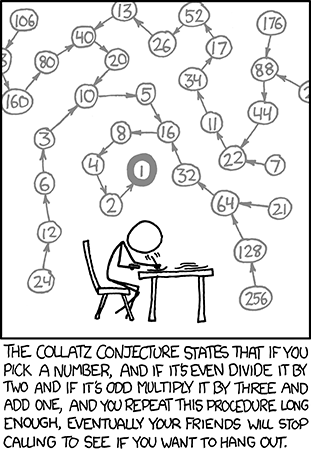
\includegraphics[width=0.8\textwidth]{collatz.png} \\
\tt{http://xkcd.com/710/}
\end{center}
%\end{figure}


\end{minipage}

